\documentclass[12pt,a4paper,oneside]{report}
\usepackage{latexsym}
\usepackage{amsmath}
\usepackage{amsfonts}
\usepackage{textcomp}
\usepackage{graphicx}
\usepackage{fancyhdr}
\usepackage{subfigure}
\usepackage{cite}
\usepackage{wrapfig}
\usepackage{rotating}
\usepackage{longtable}
\usepackage{listings}
\usepackage{dirtree}
\usepackage{minted}

\linespread{1.5}
\setlength{\headheight}{15pt}

\begin{document}

\newminted[pythoncode]{python}{
autogobble=true,
fontfamily=tt,
fontsize=\footnotesize,
linenos=false,
numberblanklines=true,
frame=lines,
tabsize=4
}

\pagenumbering{roman}

\pagestyle{empty}
\thispagestyle{empty}
\centerline{\huge \bf REST API Services using Django }
\vskip .05in
\vskip .05in
%\centerline{\huge \bf  Your Thesis}
\vskip .2in
\centerline{\it A thesis submitted to the department of }
\vskip .1in
\centerline{\it \textbf{Computer Science \& Engineering}}
\centerline{\it of}
\centerline{\it \textbf{International Institute of Information Technology, Bhubaneswar}}
\vskip .1in
\centerline{\it in partial fulfilment of the requirements}
\centerline{\it for the degree of}
\vskip .2in
\centerline{\bf \textit{Bachelor of Technology}}
\vskip .2in
\centerline{\it by}
\vskip .1in
\centerline{ \bf \textit{ Bhushan Prakash Khanale }}
\centerline{ \small \textit{ (B516025) }}
\vskip .1in
\centerline{ \textit{under the supervision of }}

\centerline{ \bf \textit{Harshad Mulmuley \& Prof. Tapan Kumar Sahoo}}
\vskip .4in

\begin{center}

\includegraphics[scale=0.75]{ch0/IIITlogo.png}\\
{{\bf{Department of Computer Science and Technology}} }\\
{{\bf International Institute of Information Technology Bhubaneswar}}\\
{{\bf Bhubaneswar Odisha - 751003, India} }\\
\end{center}

\centerline{\Large{\bf Undertaking}}
\vspace{1cm}

I declare that the work presented in this thesis titled
\textit{REST API Services using Django}, submitted to the Department of
Computer Science and Engineering, International Institute of Information
Technology, Bhubaneswar, for the award of the Bachelors of Technology degree
in the Computer Science and Engineering, is my original work. I have not
plagiarized or submitted the same work for the award of any other degree.
In case this undertaking is found incorrect, I accept that my degree may be
unconditionally withdrawn.

\vspace*{0.5in}
\begin{flushright}
Bhushan Prakash Khanale\\
B516025
\end{flushright}

\thispagestyle{empty} 
\begin{minipage}{.1\linewidth}
\hspace*{-1.8cm}
\vspace*{-1.8cm}
%\includegraphics[height=2.2cm]{ch0/NITlogo}

\includegraphics[scale=0.65]{ch0/IIITlogo.png}
\end{minipage}
\hspace{.2cm}
\begin{minipage}{.9\linewidth}
%\begin{flushleft}
{\Large
%\textsf{Department of Computer Science and Engineering\\
\textbf{International Institute of Information Technology Bhubaneswar\\}}
{\large
\text{Bhubaneswar Odisha -751 003, India.}}
\textmd{$\quad$www.iiit-bh.ac.in}
%\end{flushleft}
\end{minipage}

\vspace{.35in}
%\begin{flushleft}
%
%	\fontsize{12}{10}
%	\selectfont
%		\textbf{Dr. Professors Name}\\
%%\begin{small}
%	\fontsize{10}{10}
%	\selectfont
%		Professor 
%%\end{small}
%\end{flushleft}
\fontsize{12}{14}
\selectfont
\begin{flushright}
May 07, 2019
\end{flushright}
\vspace{1.0in}

\centerline{\Large{\bf Certificate}}
\vspace{1cm}
%\fontsize{14pt}{16.8pt}
%\begin{large}
\noindent
This is to certify that the work in the thesis entitled
{\it REST APIs for DB services using Django } by {\it Bhushan Prakash Khanale}
is a record of an original research work carried out by her under my
supervision and guidance in partial fulfillment of the requirements for
the award of the degree of \textit{Bachelor of Technology} in
\textit{Computer Science \& Engineering}. Neither this thesis nor any part of
it has been submitted for any degree or academic award elsewhere.
%\end{large}
\vspace*{0.5in}

\begin{flushright}
\textbf{\textit{Harshad Mulmuley}} \\
\textbf{\textit{Senior Software Engineer}} \\
\textbf{\textit{Turtlemint Pvt. Ltd.}}
\end{flushright}
\vspace*{0.5in}
\begin{flushright} 
\textbf{\textit{Tapan Kumar Sahoo}} \\
\textbf{\textit{Associate Professor, Computer Science}} \\
\textbf{\textit{IIIT, Bhubaneswar}}
\end{flushright}

\vspace{1in}
\centerline{\Large{\bf Acknowledgement}}
\vspace{.75cm}
\noindent The elation and gratification of this seminar will be incomplete
without mentioning all the people who helped me to make it possible, whose
gratitude and encouragement were invaluable to me. I would like to thank God,
almighty, our supreme guide, for bestowing is blessings upon me in my entire
endeavor. I express my sincere gratitude to  Harshad Mulmuley \& Prof. Tapan
Kumar Sahoo for his guidance and support and students of my class for their
support and suggestions.

\vspace*{0.5in}
\begin{flushright}
Bhushan Khanale\\
B516025, CE\\
\end{flushright}

\addcontentsline{toc}{chapter}{Abstract}
\thispagestyle{empty} 
\vspace{1.0in}
\centerline{\Large{\bf Abstract}}
\vspace{.77cm}

Most of the databases now are shared between different tenants giving it a more
complex architecture. Hence any updates being made to the database have to be
properly authenticated and verified that the changes are for that specific
tenant only. This project report introduces the process of creating a REST API
service to manage database changes with integrated authentication using Django.
REST is acronym for {\bf{RE}}presentational {\bf{S}}tate {\bf{T}}ransfer.
It is architectural style for distributed hypermedia systems. Django is an
open-source high-level Python Web framework that encourages rapid development
and clean, pragmatic design. By the features of Django and Django REST
Framework these updates to the database are are much simpler and protected.

\noindent\textbf{\textit{Keywords}:} rest, django, database
\begin{center}
% \includegraphics[scale=0.35]{ch0/textless.png}
% \caption{Textless Elements use-case example}
\end{center}

%\pare Write the abstract clearly. Ambiguity should not exist.\\\\
%\fontsize{12}{11}
%\selectfont
\vspace{.3cm}

%
%\fontsize{12}{18}

%\selectfont

\thispagestyle{empty}

%\listoffigures
%\listoftables

\linespread{1.5}
\selectfont

\tableofcontents

\pagenumbering{arabic}
\pagestyle{fancy}

\renewcommand{\chaptermark}[1]{\markboth{#1}{}}
\renewcommand{\sectionmark}[1]{\markright{\textbf{Chapter\thechapter}}}

\chapter{Introduction}

In any service dealing with the database becomes extremely important to
have a constant database structure in place before moving on towards the
business logic. In Django we define the service in terms of \texttt{app},
\texttt{models}, \texttt{views} and \texttt{services}. These four parts
represent the core logic service.
\texttt{Views} take care of the exchange of the request and response objects from APIs.
Usually when an API is called, a request object is sent to the server containing
information about the request being made. The server then has to return the
appropriate Response object which then the browser parses and outputs for the
user. This exchange between request and response is a part of Views.

\section{Background}
Turtlemint has a separate database which records most of the things related to
insurance policy issuance. This data is very volatile and is expected to change
every month. Due to this, it becomes harder to change the database every time
there is a change in the information. To handle this issue, the purpose of the
project is to create a new service which would wrap the information change in
terms of database calls and let the user seamlessly update the information.

\section{Significance}
The new service will be able to handle all information changes related to the
database. Moreover, the service would have an integrated authentication and
authorization which allows multiple users to use this service at a time.
Previously, someone from the development team had to intervene with the data
team to manually create database queries and update accordingly. This process
was not only time-consuming but also was inefficient. The new service would
solve this issue and would allow the data team itself to update the database.

\section{Method used}
The service is built using Django and Django Rest Framework (DRF) which are
two Python packages built for faster development of database-driven web
applications. Django is also open-source and allows users to modify the
report, modify any bugs if they found any. This helps for long term
support applications. Django has three major parts: \texttt{models},
\texttt{views} and \texttt{templates}. Models are used to create database
schema, views contain the business logic and templates are used for user
interface.

\section{Limitations}
Django being open-source does help in most issues. Although, since Django was
built to reduce the development time significantly it might still not have
all features of a system with independent database architecture. Django also
introduces the concept of migrations which are a set of database schema changes
maintained as a set of files. These migrations can be difficult to manage if
an application is prone to a lot of database changes.

\section{Project Structure}
Django has already defined its project structure. Every Django project has some
applications. Every application represent set of logic related to one purpose
or business objective. A project can have any number of applications inside
it. There is a common \texttt{settings.py} file which is used for managing
settings for all applications. The basic structure of the project can be
represented as below:

\dirtree{%
.1 project.
.2 settings.py. 
.2 app1.
.3 models.
.3 views. 
.3 templates. 
.2 app2.
.3 models.
.3 views. 
.3 templates. 
}

\chapter{Preliminary}
There are three important parts of this project:
\begin{itemize}
    \item Django (for API developement)
    \item Postgresql (for database requirements)
    \item Social Auth (for authentication)
\end{itemize}

\section{Django}
Django takes care of integrating the database, authentication and authorization
of the application. For this, Django asks us to construct each of models, views
and templates for the application. Its important to note that all of the three
parts are to be defined for every application in the project.

\subsection{Models}
Every model represents a table in the database. We will be forming up the
basic model structure and follow them throughout the entire project.
Every model can be defined in the \texttt{models.py} file which is recognized
by django or in the \texttt{models} module. The overall model structure would
look like this:

\dirtree{%
.1 project.
.2 app1.
.3 models.
.4 modela.py. 
.4 modelb.py. 
.4 modelc.py. 
.2 app2.
.3 models.
.4 modela.py. 
.4 modelb.py. 
}

\subsection{Views}
Every view represents the exchange of data between every API call. Every view
gets a request object and is expected to return a response object. The request
contains all information regarding the API call including the user who
initiated it. Also all of the required parameters for the API call are passed
in the same request object.\\
Views too can be distributed across multiple files for convenience.

\subsection{Templates}
Templates are used for the user interface which are automatically rendered by
Django in html. By default, Django comes with the \texttt{admin} template.
The admin page on Django lets user to modify any of the existing models and
settings. Multiple templates can be added representing the user interface.
The templates are also convenient in authentication since we can use variables
inside templates.

\section{Postgresql}
We've used Postgresql for out database requirements. Because postgres can
scale on high requirement environment and is one of the best options for
production databases. The postgresql can be installed as a separate package
and is available on all platforms including Linux, Windows and MacOS making
it ideal for deployment and development purpose.

Postgres related settings can be configured inside \texttt{settings.py} file
inside project directory. We can also specify the requirements as a part of the
environemt file to avoid exposing the credentials. The database setting is
generic in Django meaning you can use the database identically as any other
database driver. Hence, it is very easy to switch between database if we ever
wanted to.

\section{Social Auth}
For authentication there is a separate package known as
\textit{Python Social Auth} which takes care of our social authentication.
Social authentication is important because many users now try to avoid
remembering username and password and hence, using one of the social auth
method will bypass the need to remember usernames and passwords. This
authentication is based on one of the social media platforms including Google,
Facebook, Twitter, etc. These platforms proving authentication flow known as
\textit{OAuth}. The common user fields like email address, name are
automatically obtained from these platforms and a \textit{token} is created
for the user to communicate with the application.

Everyone in Turtlemint have thier email with domain \textit{turtlemint.com}
which lets us use Google OAuth2 to authenticate the user before logging it
on our application. The email address and name is obtained from Google and
appropriate permissions are issued to the user based on his access level.

\chapter{Project Architecture}

\section{An overview of the project archituecture}
The project objective is to ease the process of updating and managing the
database with proper authorization for the users. This adds up to few main
components of the project which are:

\begin{itemize}
    \item Database tables
    \item CRUD operations
    \item User permissions
\end{itemize}

\subsection{Database tables}
Currently in Turtlemint the entire database in nosql MongoDB. Hence, the first
challenge is to convert these nosql tables into relational postgres tables and
import all data from the previous database to current database. The number of
such tables is huge and hence some scripts are generated to copy the previous
database tables into the current ones. We will take a look at these scripts
later in the models section.

\subsection{CRUD operations}
Every table or model in a database has some basic CRUD (Create, Read, Update,
Delete) operations associated with it. These are declared in the models class
itself to avoid rewriting them again in the business logic. These operations
handle the basic interation with the database and can be used anywhere in the
project scope.

\begin{pythoncode}
from django.db import models

def create(**kwargs):
    turtlemint_model.objects.create(**kwargs)

def read(**kwargs):
    turtlemint_model.objects.get(**kwargs)

def delete(**kwargs):
    turtlemint_model.objects.get(**kwargs).delete()

class turtlemint_model(models.Model):
    """
    Model representing turtlemint meta information.
    """
    key = models.CharField(max_length=100, unique=True, blank=True)
    name = models.CharField(max_length=100)
    description = models.TextField(max_length=100)
    ...
\end{pythoncode}

\subsection{User permissions}
There are usually two ways we can create users based on their permission
levels. One of the ways is to use Django's inbuilt \texttt{groups} which can
create seperate groups for users and every group would then have a dedicated
level of permission which would then be applied for every user in that group.
This process is handy for most of the simple applications which don't have
to deal with a lot of different user sets.

The other way is to define a \texttt{CustomUser} model overriding Django's
inbuilt \texttt{User} model. This gives us much more freedom over the user
characterstics and can then be used with different permission classes. As
mentioned above, Django have some of the permission classes already defined
while other can be manually created.

\begin{pythoncode}
class TurtlemintUser(AbstractBaseUser):
    """
    This class represents Custom User Model,
    that overrides django builtin User model
    """
    key = models.CharField(max_length=100, unique=True, blank=True)
    email = models.EmailField(
        verbose_name='email address',
        max_length=255,
        unique=True,
    )
    first_name = models.CharField(max_length=100, blank=True)
    last_name = models.CharField(max_length=100, blank=True)
    password = models.CharField(max_length=200, blank=True)
    ...
\end{pythoncode}

Every user has some sort of permissions associated with it. These permissions
are used to determine whether a user can interact with a certain database table
or not. Django in itself provides \texttt{PermissionClasses} which can be used
to determine the scope for the user. We can also create custom permissions
classes by extending the \texttt{BasePermission} class and overriding
appropriate class methods.

An example of a \texttt{CustomPermission} class can be given as below:
\begin{pythoncode}
from rest_framework.permissions import BasePermission
class IsSuperAdmin(BasePermission):
    """
    Allows access only to super admin users.
    """
    def has_permission(self, request, view):
        return bool(request.user and request.user.is_staff)
\end{pythoncode}

\section{Business Logic}
Most of the archituecture is covered in the above sections, there are still
some organization specific requirements which are to be fullfilled. These are
all considered under business logic. The business logic just represents the
actual code written to complete an objective or requirement imposed by the
organization. At Turtlemint, we've number of requirements for which we need
to split the project into several modules.

The most of the business logic should go in the \texttt{services/} directory.
This is not a Django specific module, but is actually user defined. Hence, the
name can be changed to whichever suitable. The business logic should be as
isolated as possible since then it will be easier to write unittests against
it. Unittests are written to check for every possible scenario and to check if
its response is the one which is expected. Having a good code coverage will
help maintainers in matintaining the software in long run.

\chapter{Development Process}

\section{Initial setup}
The initial project setup consists of various steps including setting up the
local development environment, Python and its dependencies and finally the
initial Django project template. Django project can be initialized using the
command \texttt{django-admin startproject mysite}. The command will create a
new directory named \texttt{mysite} in your current directory. It represents
the Django project. Once the project has been initialized, we need to create
a new application within the project by the command
\texttt{python manage.py startapp appname}. This will create a new directory
inside your project directory representing a Django application.

Once the application has been initialized, we can move towards the actual
development of the application. This process involves several steps including
creating models, views, serializers, services etc. But before that it is
important to setup the project settings correctly. You can select the database
driver of your choice and modify the \texttt{settings.py} file in your project
directory.

\section{Create models}
As mentioned previously before, models represent the database tables. These
models can be defined in seperate files or can be defined in a single file
named \texttt{models.py} as required. Before starting to write the actual
implementation it is critical to design and write the database schema first.
Django provides you with an inbuilt \texttt{Model} class which you can extend
to write you own models. Most of the methods in the \texttt{Model} class are
reusable and hence we don't have to write custom methods for every class.

\begin{pythoncode}
# models/turtlemint_model.py

class TurtlemintModel(models.Model):
    """
    Model representing Turtlemint meta model.
    """
    key = models.CharField(max_length=100, unique=True, blank=True)
    name = models.CharField(max_length=100)
    description = models.TextField(max_length=100)
    logo = models.CharField(max_length=200, null=True, blank=True)
    home_url = models.CharField(max_length=200, null=True)
    support_email = models.EmailField(blank=True, null=True)
    ...
\end{pythoncode}

\begin{pythoncode}
# models/turtlemint_insurer_model.py
    
class InsurerModel(models.Model):
    """
    Model representing insurer meta model.
    """
    key = models.CharField(max_length=100, unique=True, blank=True)
    name = models.CharField(max_length=100)
    associated_vertical = models.CharField(max_length=200, null=True)
    logo = models.CharField(max_length=200, null=True, blank=True)
    home_url = models.CharField(max_length=200, null=True, blank=True)
    support_email = models.EmailField(blank=True, null=True)
    ...
\end{pythoncode}

To make reflect these models into our database we need to create Django
migrations. These migrations can be created using the command
\texttt{python manage.py makemigrations}. This would create a new directory
inside you app representing the database queries. Internally, Django parses
the changes made to the models into their equivalent database queries. These
created migrations are then ran using the command
\texttt{python manage.py migrate} to reflect them in your database.

\section{Create serializers}
Serializers allow complex data such as querysets and model instances to be
converted to native Python datatypes that can then be easily rendered into
JSON, XML or other content types. Serializers also provide deserialization,
allowing parsed data to be converted back into complex types, after first
validating the incoming data.

Every models should have its own serializer, representing the construction of
the JSON object throught the model fields. Serializers are extremely useful
to return the JSON object instantly without having to construct it manually.
Django allows us to define the fields we want the serializer to construct the
JSON with. Also, we can have multiple serializers for a model if we want a
separate response based on the request.

An example of serializer can be given as below:
\begin{pythoncode}
class TurtlemintModelSerializer(serializers.ModelSerializer):
    """
    Serializer for the TurtlemintModel.
    """
    class Meta:
        model = TurtlemintModel
        fields = ['id', 'key', 'name', 'description', 'language'...]
\end{pythoncode}

\section{Add CRUD operations}
Every model should have its own each of CRUD methods. These methods will be
commonly shared and used by the views and business logic. Also these functions
should be unittestable to make sure that they are doing exactly what is
intended of them. Hence it is critical that these methods should be an early
part of the development process.

\section{Add views}
Views take care of accepting the request and returning the appropriate
response. These are defined inside the \texttt{views} module and can be split
into various files and classes. Views can be written in two ways, having a
separate class to handle all requests including GET, POST, DELETE, etc for a
single endpoint or to have indivitual view methods for each type of request.
Django supports both ways equally and hence any method should suffice based
on the development need.

Examples of views:
\begin{pythoncode}
class TurtlemintView(APIView):
    """
    Turtlemint view.
    """
    def get(self, request):
        return Response(Turtlemint.get_data(request.data),
                        status_code=status.HTTP_200_OK)
    def post(self, request):
        responseTurtlemint.update(request.data)
        if response['success']:
            return Response(response, status_code=HTTP_200_OK)
        return Response(response, status_code=HTTP_400_BAD_REQUEST)
\end{pythoncode}

To make this operational for an endpoint, we need to add an entry in
\texttt{urls.py} file for the same.

\begin{pythoncode}
# urls.py
urlpatterns = [
    ...
    path('api/v1/turtlemint/meta', TurtlemintView.as_view()),
    ...
]
\end{pythoncode}

The views also link to the business logic for that API, this will be covered
in the next chapter as a part of Turtlemint and its requirements.

\section{API testing}
The APIs can be manually tested using any framework like Postman. Django also
provides a nice UI to be able to send requests. At turtlemint we've a culture
of using Postman extensively for API testing and we've followed the same.
Although, apart from the Postman tests it is also necessary to construct
unittests and view tests using Django's \texttt{TestCase} class.

\subsection{Unittests}
Django provides an extended version of \texttt{unittest.TestCase} class which
automatically creates a test database and destroys it at the end of test
execution cycle. Also every test is ran as a separate transaction hence
allowing the database to rollback automatically once some error is encountered
in the tests.

As per the default behaviour of unittest, every test file should start with
\texttt{test} prefix and should correctly represent the file under testing.
Tests can be written as a part of a class which may include \texttt{setUp}
and \texttt{taildown} function to represent to initate, and clear some process
at the start and the end of the test execution.

\begin{pythoncode}
class TestTurtlemintModel(TestCase):
    def setUp(self):
        # Run something before running the testcase
        self.model = TurtlemintModel
    def test_get_records_count(self):
        # Get the output from the method under test
        result = get_records_count(self.model)
        self.assertEqual(result, 1) # 1 representing expexted result
\end{pythoncode}

\subsection{Postman tests}
Unittests are always preferred, but for some reason if we need some sort of
integration tests then postman tests can be written. Postman is an application
used for API collection management. It introduces a lot of features including
one to write tests for the API collections. For every request you can mock
the expected response and check if the response is correct or not. Although
this might be helpful in some cases, we initially wrote some tests here but
later due to introduction of unittests we dropped this process.

\begin{figure}
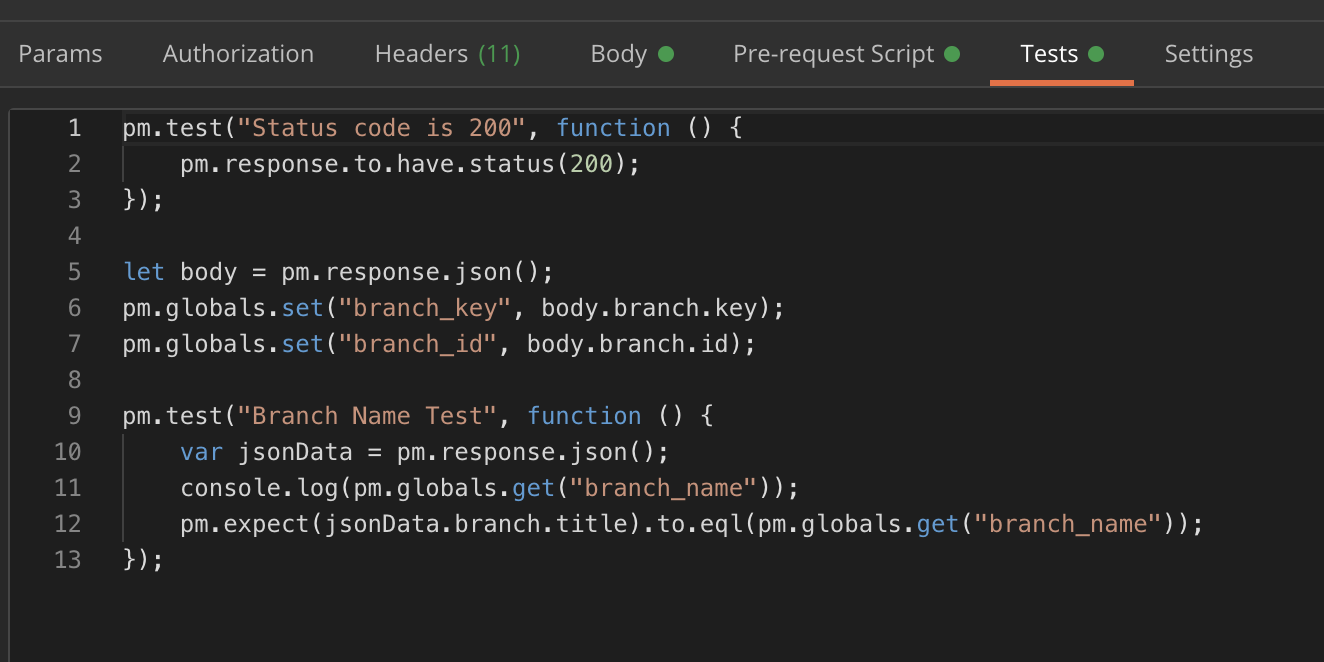
\includegraphics[width=\textwidth]{ch4/postman_test.png}
\caption{Sample Postman testcase}
\end{figure}


% \renewcommand{\chaptermark}[1]{\markboth{{#1}}{\section}}
% %\renewcommand{\sectionmark}[1]{\markright{\MakeUppercase{#1}}{}}


% \rhead{\textit{Bibliography}}
% \lhead{}

% \addcontentsline{toc}{chapter}{Bibliography}
% \bibliographystyle{unsrt}
% \bibliography{refer}
% \nocite{*}
% \cleardoublepage

\end{document}
